%!TEX root = ../paper.tex
\chapter{效果}
	\section{星座图}
		\par 在电脑上,如果程序正常运行,则可以在接收端看到如图\ref{fig:dvbt_rx_map_1}和\ref{fig:dvbt_rx_map_2}星座图。
		\begin{figure}[htp]
			\centering
			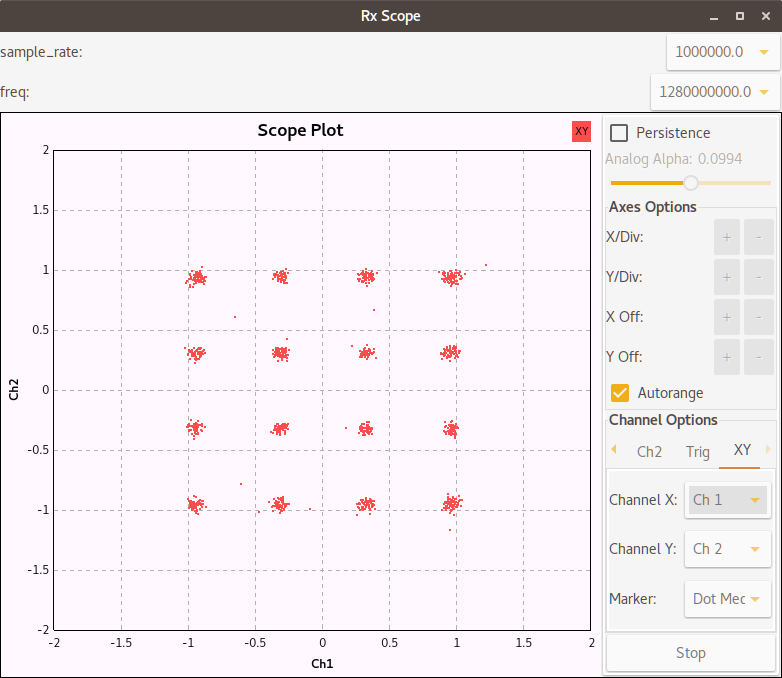
\includegraphics[width=13cm]{figures/dvbt_rx_map_1.png}
			\caption{DVB-T接收端星座图}
			\label{fig:dvbt_rx_map_1}
		\end{figure}
		\begin{figure}[htp]
			\centering
			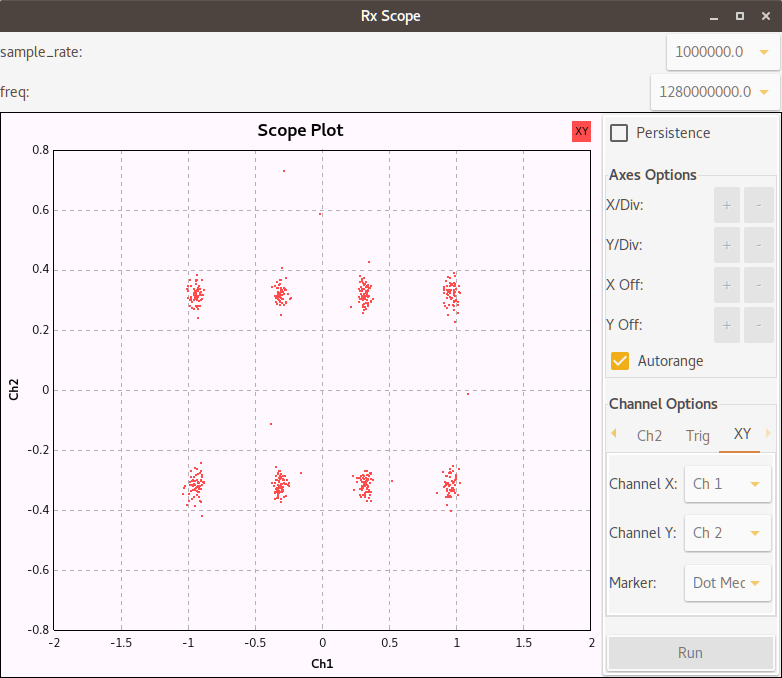
\includegraphics[width=13cm]{figures/dvbt_rx_map_2.png}
			\caption{DVB-T接收端星座图}
			\label{fig:dvbt_rx_map_2}
		\end{figure}
	\section{波形}
		\par 有如下几种方式查看输出波形:
		\par $\bullet$ 使用GNU Radio构建一个简易的频谱仪
		\par $\bullet$ 使用示波器
		\par 带宽为2MHz时波形如图\ref{fig:dvbt_BW_2MHz}所示,带宽为5MHz时波形如图\ref{fig:dvbt_BW_5MHz}所示。
		\begin{figure}[htp]
			\centering
			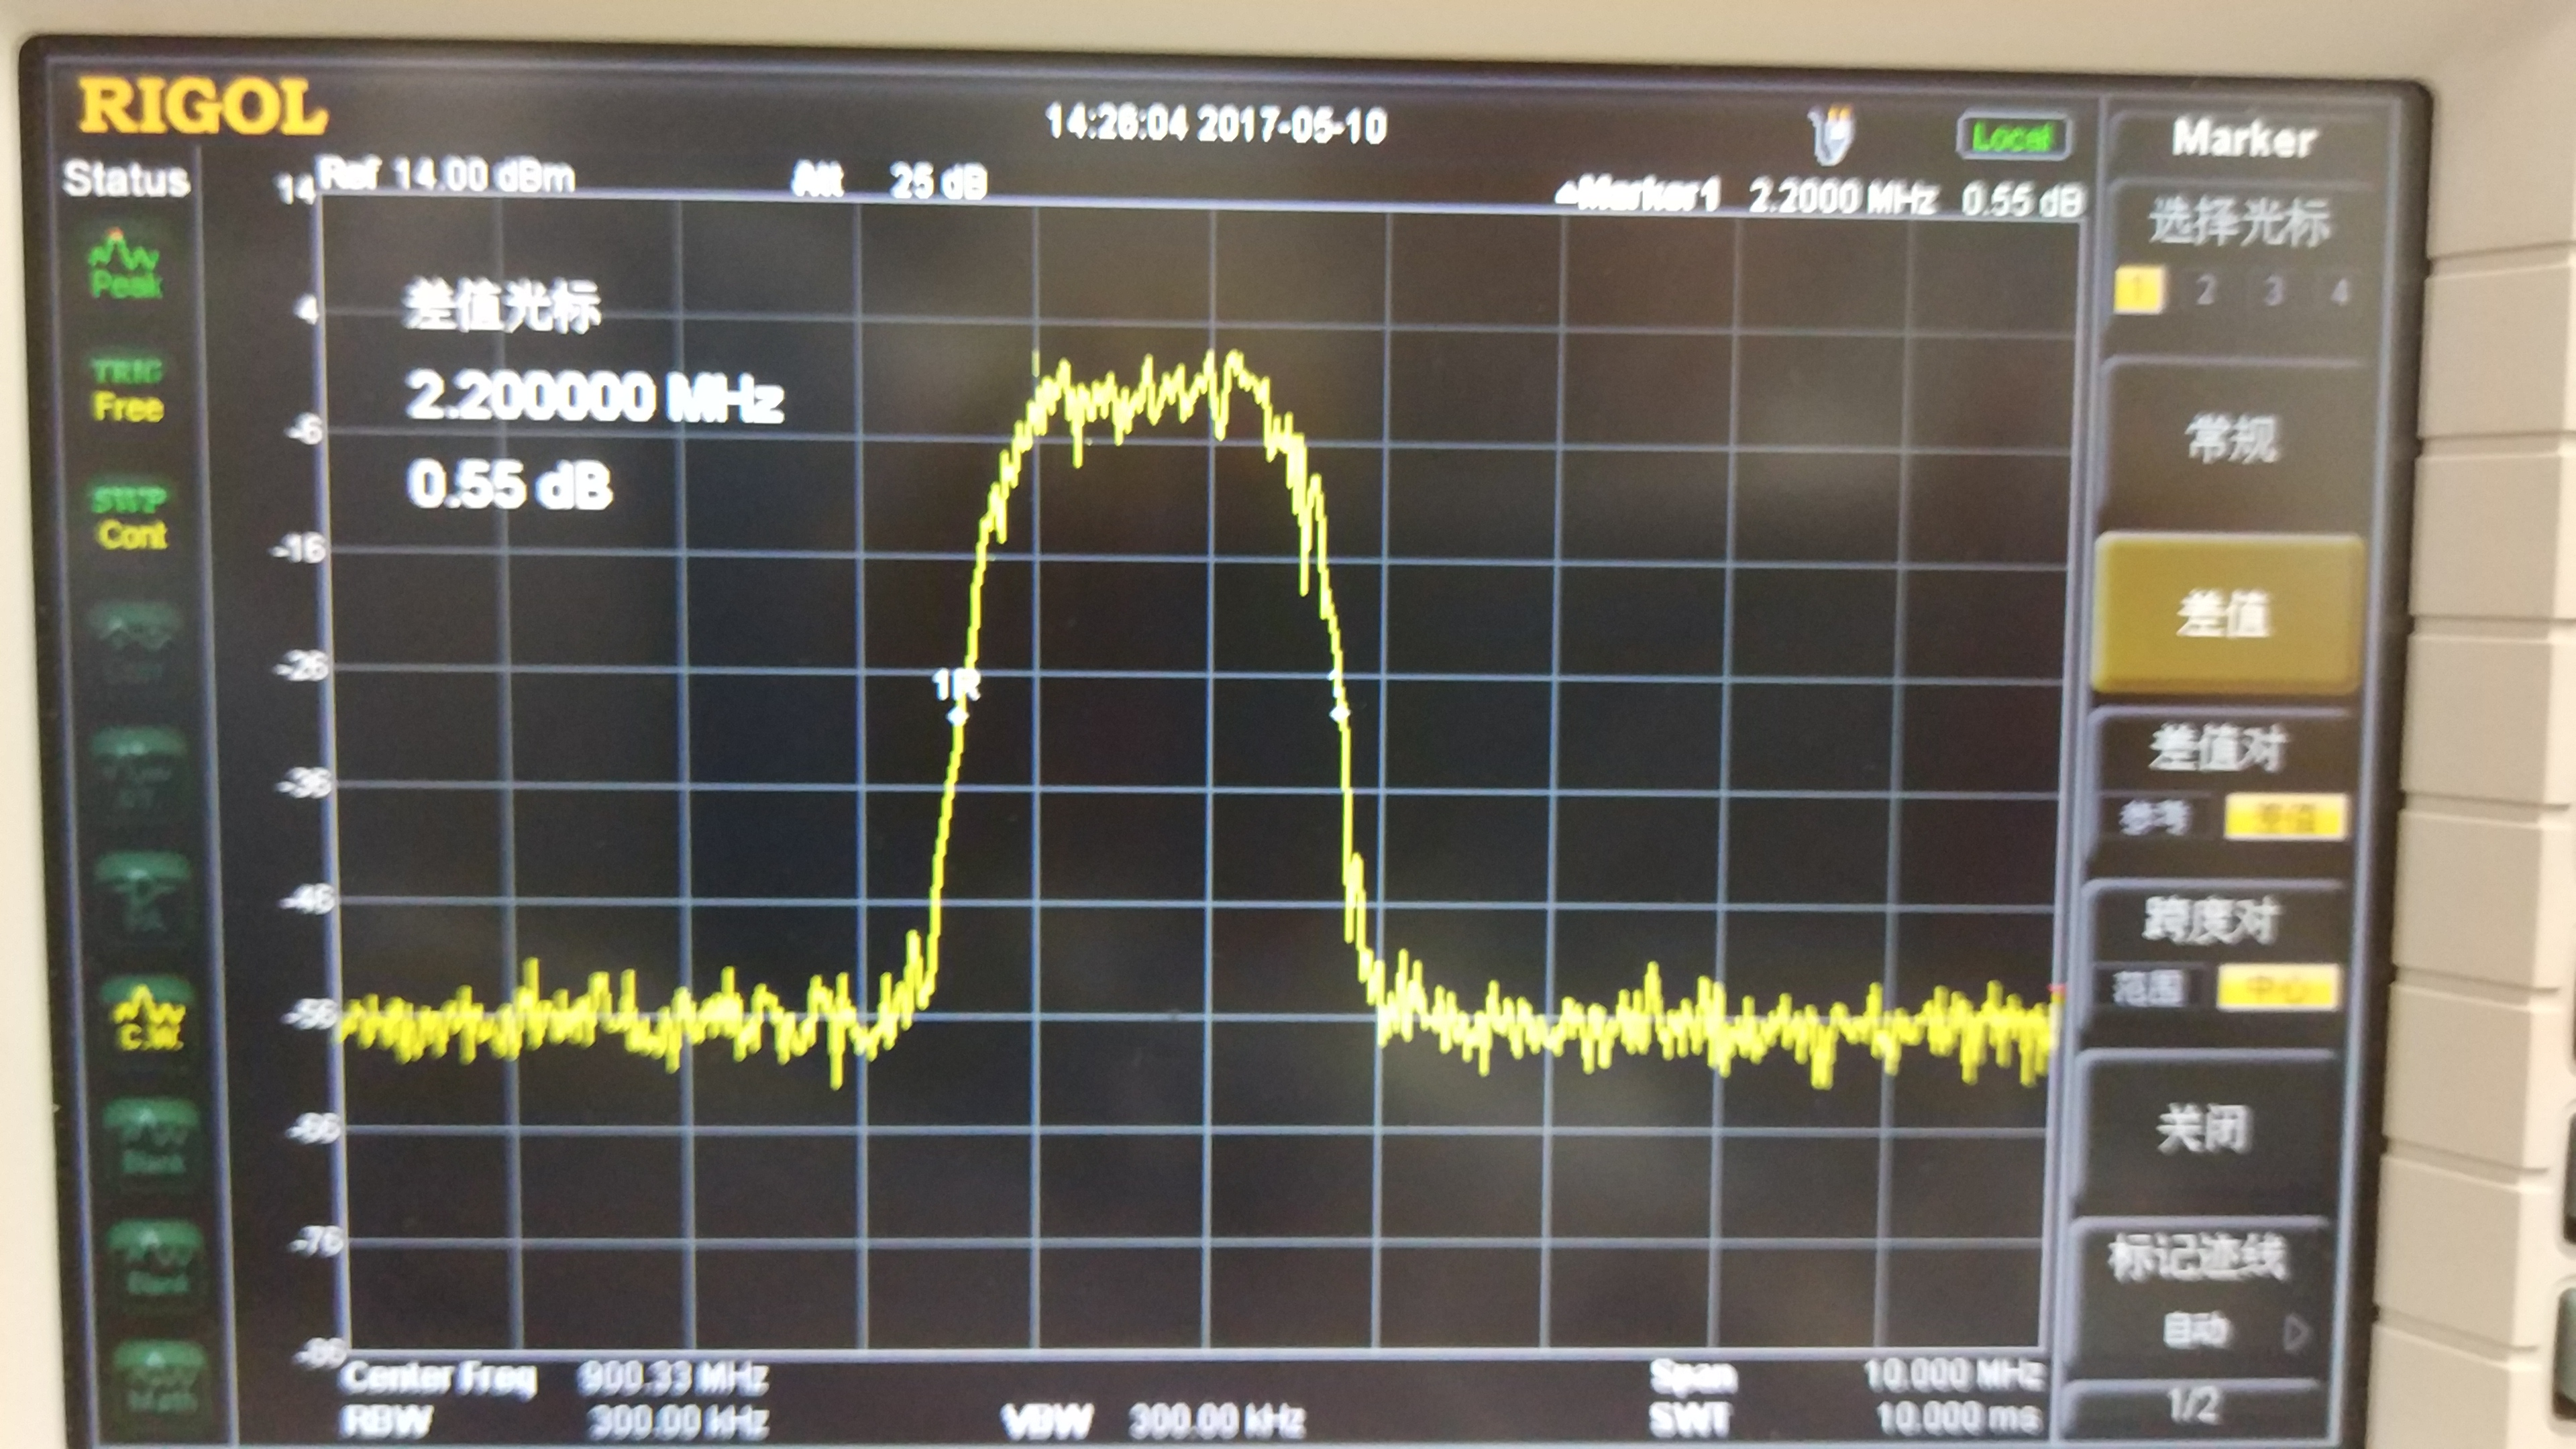
\includegraphics[width=13cm]{figures/dvbt_BW_2MHz.jpg}
			\caption{带宽为2MHz时示波器波形}
			\label{fig:dvbt_BW_2MHz}
		\end{figure}
		\begin{figure}[htp]
			\centering
			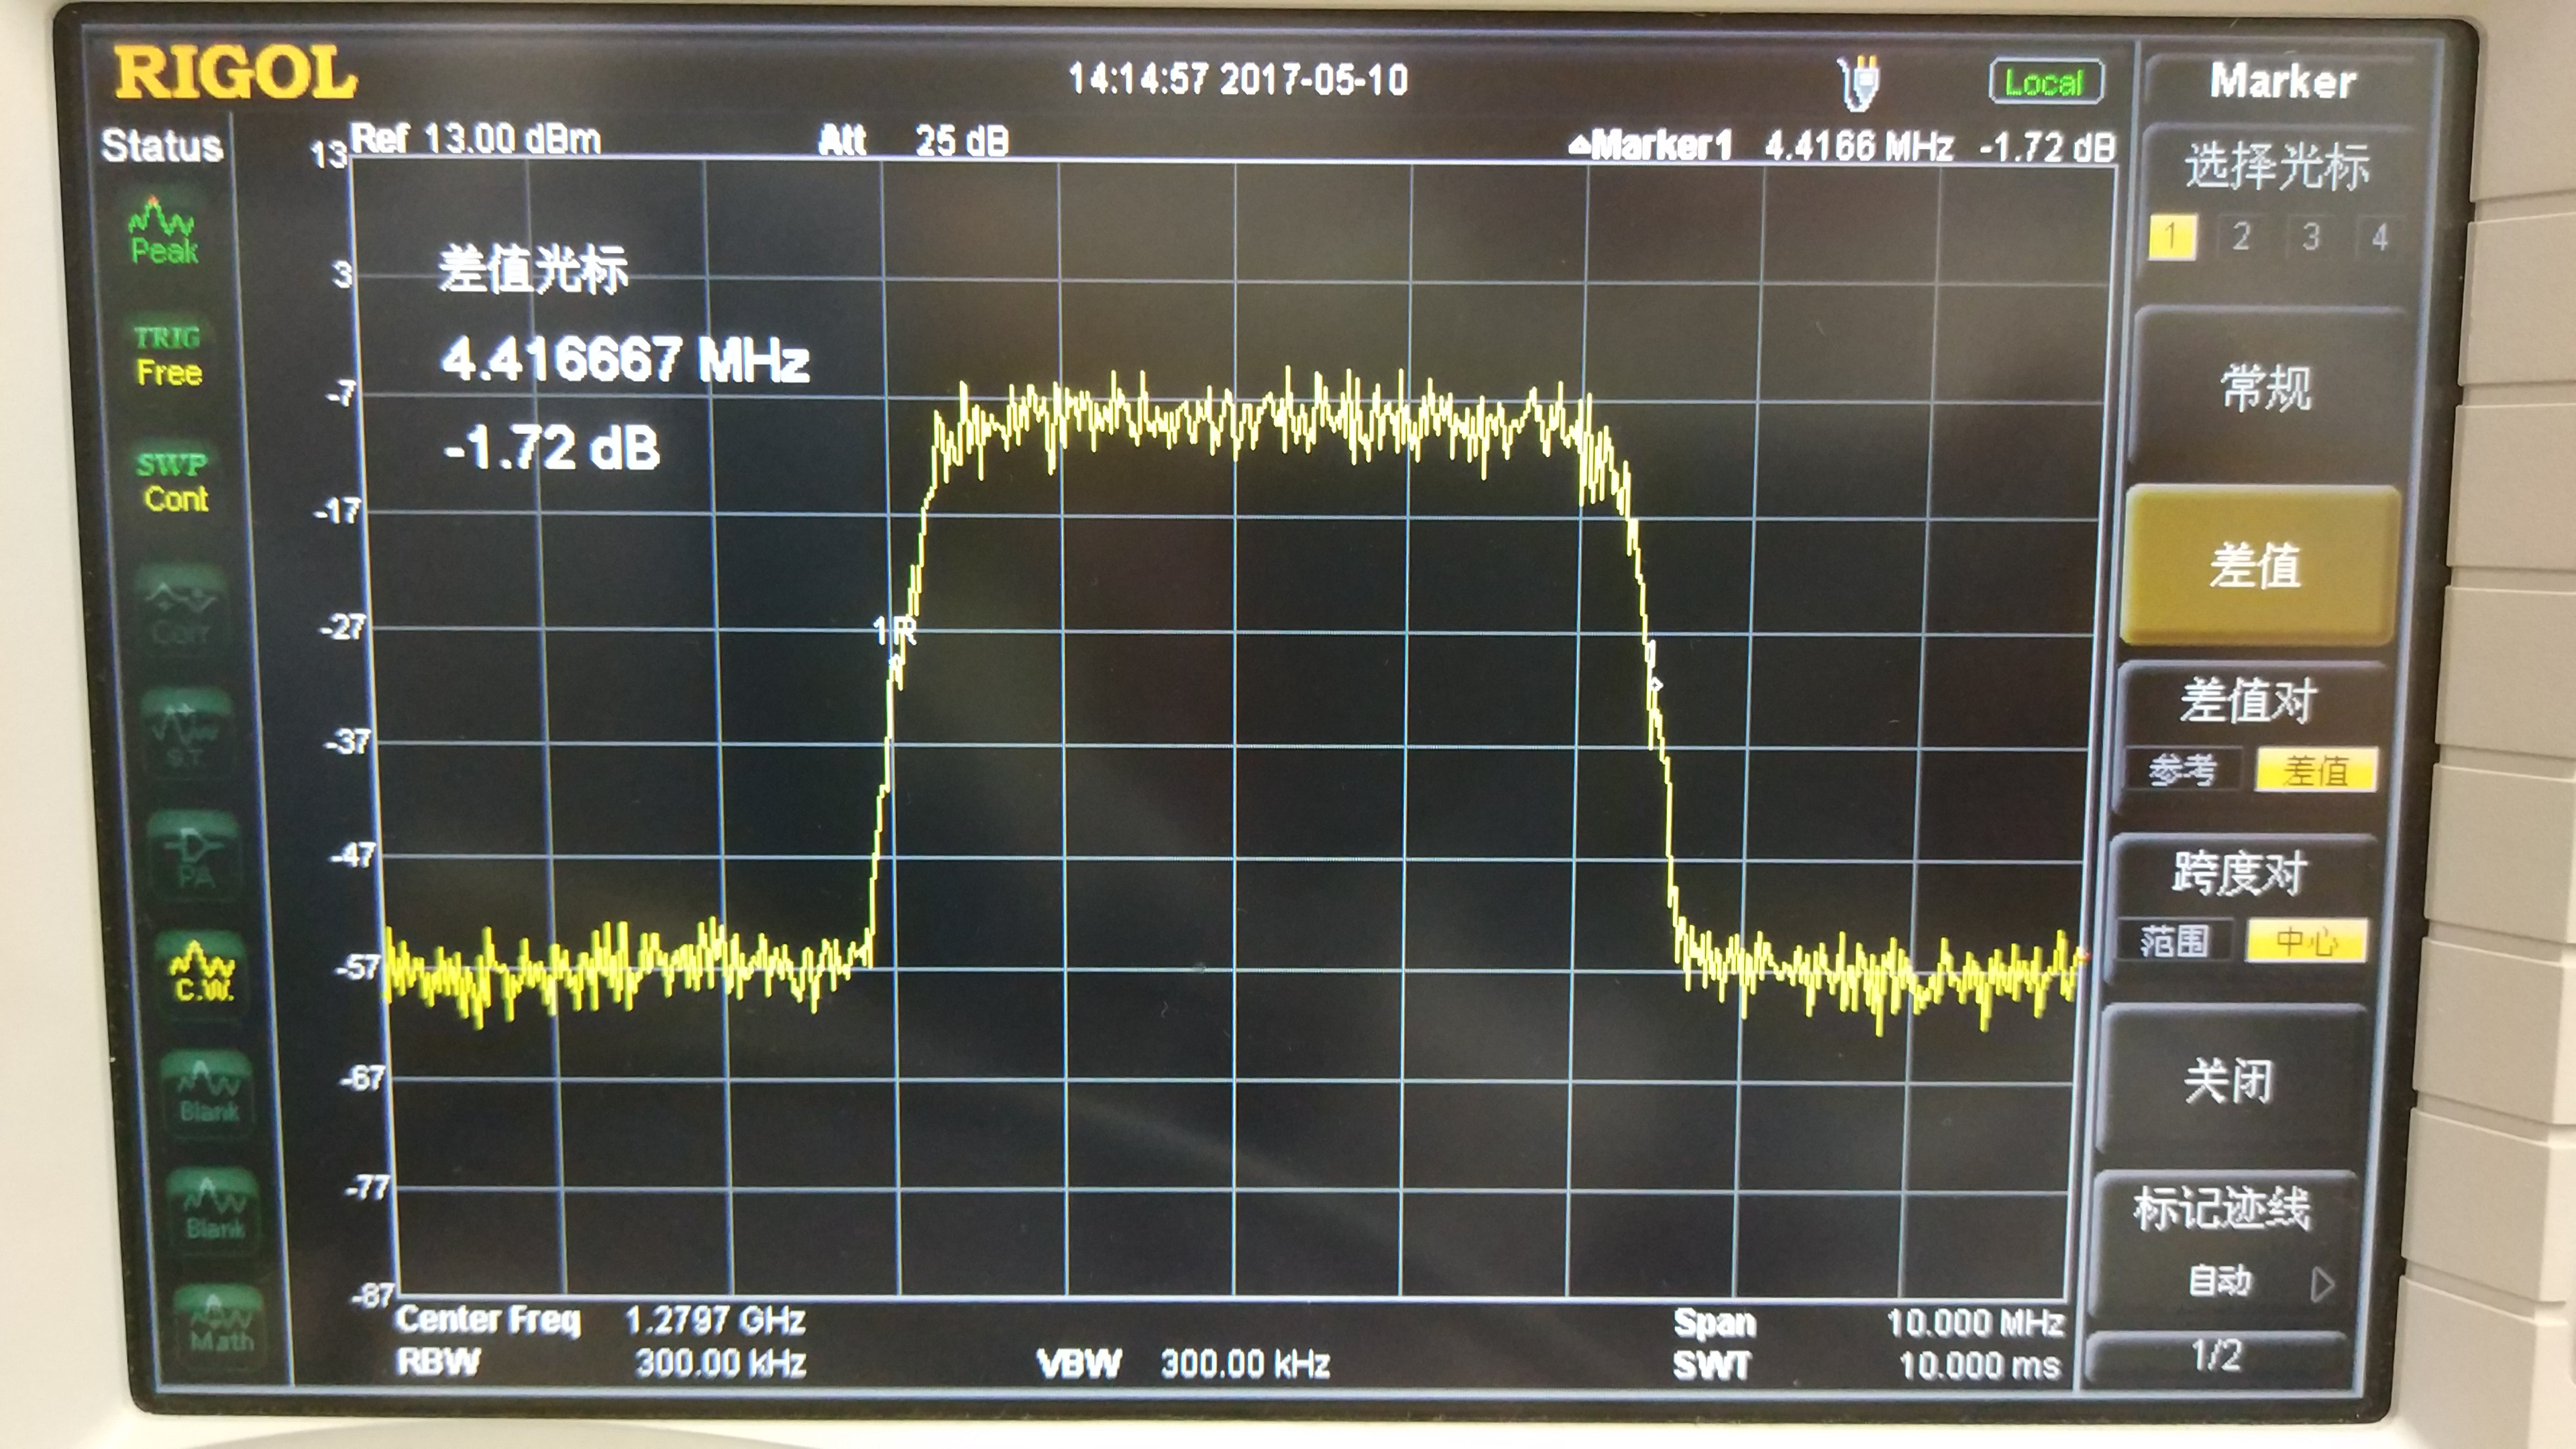
\includegraphics[width=13cm]{figures/dvbt_BW_5MHz.jpg}
			\caption{带宽为5MHz时示波器波形}
			\label{fig:dvbt_BW_5MHz}
		\end{figure}
		\par $\bullet$ 使用gqrx
	\section{距离}
		\par 收发端之间距离较近时可以在当前目录下看到生成的\lstinline[language=sh]{test_out.ts}文件,使用VLC或者Mplayer可以播放出视频,如图\ref{fig:dvbt_rx_TS}。
		\begin{figure}[htp]
			\centering
			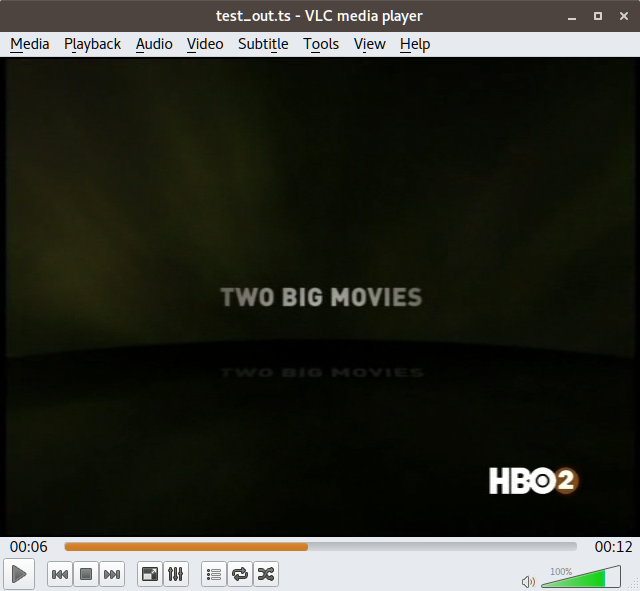
\includegraphics[width=13cm]{figures/dvbt_rx_TS.png}
			\caption{视频输出}
			\label{fig:dvbt_rx_TS}
		\end{figure}	
		\par 由于USRP的输出功率(约1W),信号能传播大约一间屋子的距离(约5米),超过这段距离将会出现以如图\ref{fig:dvbt_rx_2MHz_ranged_2}星座图以及如图\ref{fig:dvbt_rx_TS_broken}视频播放的失真。
		\begin{figure}[htp]
			\centering
			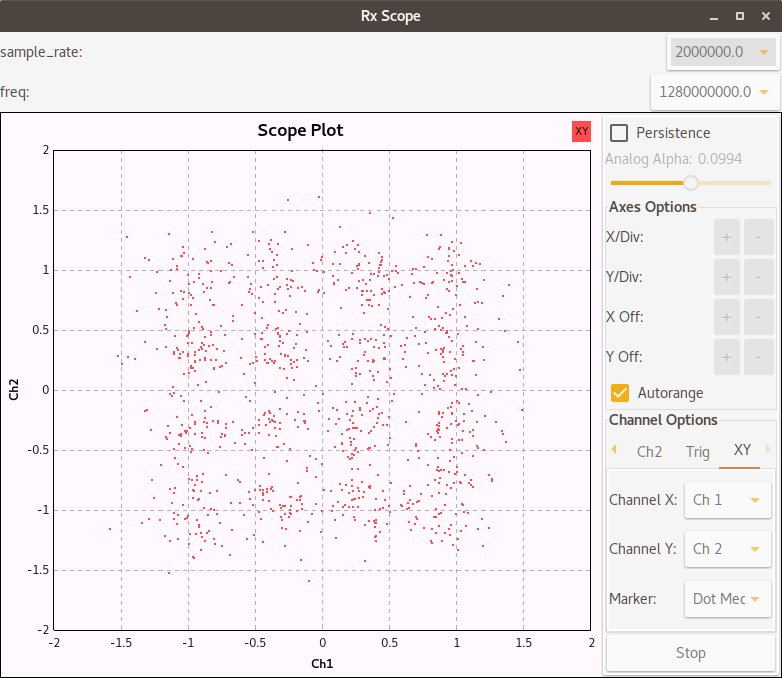
\includegraphics[width=13cm]{figures/dvbt_rx_2MHz_ranged_2.png}
			\caption{约5m处星座图}
			\label{fig:dvbt_rx_2MHz_ranged_2}
		\end{figure}
		\begin{figure}[htp]
			\centering
			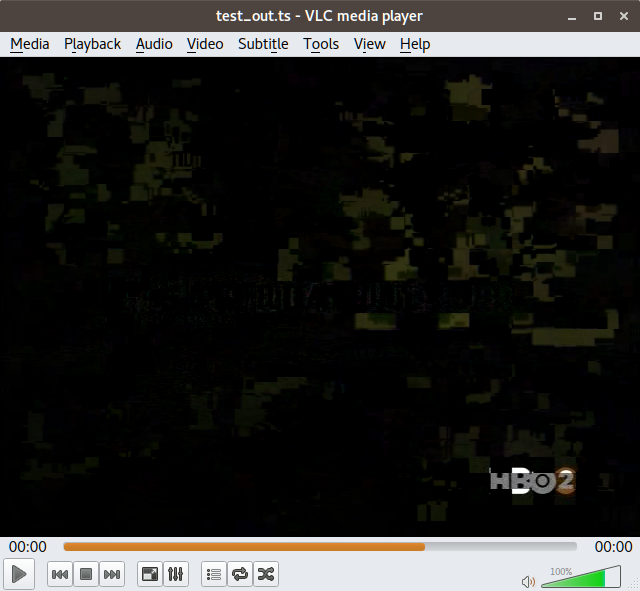
\includegraphics[width=13cm]{figures/dvbt_rx_TS_broken.png}
			\caption{约5m处视频解码}
			\label{fig:dvbt_rx_TS_broken}
		\end{figure}
	\section{树莓派发射}
